% Options for packages loaded elsewhere
\PassOptionsToPackage{unicode}{hyperref}
\PassOptionsToPackage{hyphens}{url}
%
\documentclass[
]{article}
\usepackage{lmodern}
\usepackage{amssymb,amsmath}
\usepackage{ifxetex,ifluatex}
\ifnum 0\ifxetex 1\fi\ifluatex 1\fi=0 % if pdftex
  \usepackage[T1]{fontenc}
  \usepackage[utf8]{inputenc}
  \usepackage{textcomp} % provide euro and other symbols
\else % if luatex or xetex
  \usepackage{unicode-math}
  \defaultfontfeatures{Scale=MatchLowercase}
  \defaultfontfeatures[\rmfamily]{Ligatures=TeX,Scale=1}
\fi
% Use upquote if available, for straight quotes in verbatim environments
\IfFileExists{upquote.sty}{\usepackage{upquote}}{}
\IfFileExists{microtype.sty}{% use microtype if available
  \usepackage[]{microtype}
  \UseMicrotypeSet[protrusion]{basicmath} % disable protrusion for tt fonts
}{}
\makeatletter
\@ifundefined{KOMAClassName}{% if non-KOMA class
  \IfFileExists{parskip.sty}{%
    \usepackage{parskip}
  }{% else
    \setlength{\parindent}{0pt}
    \setlength{\parskip}{6pt plus 2pt minus 1pt}}
}{% if KOMA class
  \KOMAoptions{parskip=half}}
\makeatother
\usepackage{xcolor}
\IfFileExists{xurl.sty}{\usepackage{xurl}}{} % add URL line breaks if available
\IfFileExists{bookmark.sty}{\usepackage{bookmark}}{\usepackage{hyperref}}
\hypersetup{
  hidelinks,
  pdfcreator={LaTeX via pandoc}}
\urlstyle{same} % disable monospaced font for URLs
\usepackage[margin=1cm]{geometry}
\usepackage{longtable,booktabs}
% Correct order of tables after \paragraph or \subparagraph
\usepackage{etoolbox}
\makeatletter
\patchcmd\longtable{\par}{\if@noskipsec\mbox{}\fi\par}{}{}
\makeatother
% Allow footnotes in longtable head/foot
\IfFileExists{footnotehyper.sty}{\usepackage{footnotehyper}}{\usepackage{footnote}}
\makesavenoteenv{longtable}
\usepackage{graphicx}
\makeatletter
\def\maxwidth{\ifdim\Gin@nat@width>\linewidth\linewidth\else\Gin@nat@width\fi}
\def\maxheight{\ifdim\Gin@nat@height>\textheight\textheight\else\Gin@nat@height\fi}
\makeatother
% Scale images if necessary, so that they will not overflow the page
% margins by default, and it is still possible to overwrite the defaults
% using explicit options in \includegraphics[width, height, ...]{}
\setkeys{Gin}{width=\maxwidth,height=\maxheight,keepaspectratio}
% Set default figure placement to htbp
\makeatletter
\def\fps@figure{htbp}
\makeatother
\setlength{\emergencystretch}{3em} % prevent overfull lines
\providecommand{\tightlist}{%
  \setlength{\itemsep}{0pt}\setlength{\parskip}{0pt}}
\setcounter{secnumdepth}{5}
\usepackage{float} \floatplacement{figure}{H}
\usepackage{float}
\ifluatex
  \usepackage{selnolig}  % disable illegal ligatures
\fi

\author{}
\date{\vspace{-2.5em}}

\begin{document}

\renewcommand{\figurename}{Supplementary Figure}
\renewcommand{\tablename}{Supplementary Table}
\pagenumbering{gobble}

\newpage

\hypertarget{supplementary-figures}{%
\section*{Supplementary Figures}\label{supplementary-figures}}
\addcontentsline{toc}{section}{Supplementary Figures}

\begin{figure}
\includegraphics[width=500px]{suppl_figs/suppl_fig_refined} \caption{\textbf{Random sampling of KNN graph vertices is suboptimal compared to sampling with refinement.}
(A) Sampling with refinement leads to selection of fewer neighbourhoods
(B) Sampling with refinement leads to selection of bigger neighbourhoods for DA testing, independently of the initial proportion of cells sampled
(C) Sampling with refinement generates robust neighbourhoods across initializations: for each index cell we calculate the distance from the closest index in a sampling with different initialization. The cumulative distribution of distances to the closest index is shown. The black dotted line denotes the distribution of distances between K nearest neighbors in the dataset (K=30) (NH: neighbourhood).
Neighbourhood statistics were calculated using a simulated trajectory dataset of 5000 cells. All plots show results from three sampling initializations for each proportion.}\label{fig:sup-fig-refined}
\end{figure}







\begin{figure}
\centering
\includegraphics{suppl_figs/suppl_fig_clustering.pdf}
\caption{\label{fig:sup-fig-clustering}\textbf{Graph-clustering does not faithfully capture simulated groups and differentially abundant subpopulations in a simulated continuous trajectory.}
(A) A simulated linear trajectory of 2000 single-cells generated from 5 different groups, with cells assigned to either condition `A' (left) or condition `B' (right).
(B) A Walktrap clustering of the data in (A) using the same KNN graph. Cells are coloured by Walktrap cluster identity.
(C) A Louvain clustering of the data in (A) using the same KNN graph. Cells are coloured by the Louvain clustering identity.
(D-E) Heatmaps comparing the numbers of cells in each cluster with respect to the ground truth groups in (A). Each cell is coloured by the proportion of cells from the column groups (ground truth) that are assigned to the respective cluster.}
\end{figure}







\begin{figure}
\centering
\includegraphics{suppl_figs/suppl_fig_krobustness.pdf}
\caption{\label{fig:sup-fig-robustness}\textbf{Robustness of Milo DA testing to varying K}. Distributions of DA neighbourhoods across values of K for the mouse ageing thymus (A) and human cirrhotic liver (B) data sets. Shown are the distributions of log fold-changes (y-axis) for DA (FDR 10\%) neighbourhoods using different values of K (x-axis) from 5-100, illustrating that DA testing is robust across a broad range of values of K.}
\end{figure}



\begin{figure}
\centering
\includegraphics{suppl_figs/suppl_fig_bm_threshold.pdf}
\caption{\label{fig:sup-fig-bm-threshold}\textbf{Selection of probability threshold for DA benchmarking.} Mean True Positive Rate (left) and False Discovery Rate (right) for recovery of cells in simulated DA regions as a function of probability threshold \(t\) picked to define true DA. The dashed line indicates \(t = 0.6\), that was selected for benchmarking analyses. The mean is calculated over simulations on 8 populations. Line shading indicates the standard deviation of the mean.}
\end{figure}



\begin{figure}
\includegraphics[width=500px]{suppl_figs/suppl_fig_bm_simulations} \caption{\textbf{Benchmarking DA methods on simulated data.} DA analysis performance on KNN graphs from simulated datasets of different topologies: (A) discrete clusters (1800 cells, 3 populations); (B) 1-D linear trajectory (7500 cells, 7 populations); (C) Branching trajectory (7500 cells, 10 populations).}\label{fig:sup-fig-bm-simulations}
\end{figure}



\begin{figure}
\includegraphics[width=500px]{suppl_figs/suppl_fig_signal2noise} \caption{\textbf{Variability in Milo power is explained by the fraction of true positive cells close to DA threshold} example distributions of underlying probability of Condition1 (P(C1)) for cells detected as True Positives (TP) or False Negatives (FN) by Milo. Examples for simulations on 2 populations (rows) and 3 simulated fold changes (columns) are shown.}\label{fig:sup-fig-bm-signal}
\end{figure}



\begin{figure}
\includegraphics[width=500px]{suppl_figs/suppl_fig_bm_size} \caption{\textbf{DA testing power increases with the size of the DA population} True Positive Rate (TPR) of DA detection for simulated DA regions of increasing size centered at the same centroid (Erythroid2 (A) and Caudal neuroectoderm (B)). Results for 3 condition simulations per population and fold change are shown.}\label{fig:sup-fig-bm-size}
\end{figure}



\begin{figure}
\centering
\includegraphics{suppl_figs/suppl_fig_bm_batch.pdf}
\caption{\label{fig:sup-fig-bm-batch}\textbf{Batch effect control across DA effect sizes.} True Positive Rate (TPR, left) and False Discovery Rate (FDR, right) for recovery of cells in simulated DA regions for DA populations with increasing batch effect magnitude on the mouse gastrulation dataset. For each boxplot, results from 8 populations and 3 condition simulations per population are shown. Each panel represents a different DA method and a different simulated log-Fold Change.}
\end{figure}



\begin{figure}
\centering
\includegraphics{suppl_figs/suppl_fig_bm_MNN.pdf}
\caption{\label{fig:sup-fig-bm-mnn}\textbf{In silico batch correction enhances the performance of DA methods in the presence of batch effects.} Comparison of performance of DA methods with no batch effect, with batch effects of increasing magnitude corrected with MNN, and uncorrected batch effects.}
\end{figure}



\begin{figure}
\centering
\includegraphics{suppl_figs/suppl_fig_bm_design.pdf}
\caption{\label{fig:sup-fig-bm-design}\textbf{Modelling batch effects in DA analysis with Milo.} (B) Comparison of Milo performance with (\textasciitilde{} batch + condition) or without (\textasciitilde{} condition) accounting for the simulated batch in the GLM. For each boxplot, results from 8 populations, simulated fold change \textgreater{} 1.5 and 3 condition simulations per population and fold change are shown (72 simulations per boxplot).}
\end{figure}



\begin{figure}
\includegraphics[width=500px]{suppl_figs/suppl_fig_meldVSmilo} \caption{\textbf{Comparison of Milo and MELD for abundance fold-change estimation.} (A-D) Scatter-plots of the true fold-change at the neighbourhood index against the fold-change estimated by Milo (A,C) and MELD (B,D), without batch effect (A-B) and with batch effect (magnitude = 0.5) (C-D), where \(LFC = log(p_{c'}/(1 - p_{c'}))\). The neighbourhoods overlapping true DA cells (\(p_{c'}>0.6\)) are highlighted in red. (C-D) Mean Squared Error (MSE) comparison for MELD and Milo for true negative neighbourhood (C) and true positive neighbourhoods (D), with increasing simulated log-Fold Change and magnitude of batch effect.}\label{fig:sup-fig-bm-meld}
\end{figure}



\begin{figure}
\centering
\includegraphics{suppl_figs/suppl_fig_MSE-k_vs_replicates.pdf}
\caption{\label{fig:sup-fig-msek}\textbf{Impact of replication and k selection on variance in estimates}}
\end{figure}



\begin{figure}
\includegraphics[width=500px]{suppl_figs/suppl_fig_memory} \caption{\textbf{Memory usage across the Milo analysis workflow.}
Total memory usage across the steps of the Milo analysis workflow in 4 datasets containing different numbers of cells (Gastrulation: circles, Liver: triangles, Thymus: crosses, Simulation: squares). Grey pointed denot down-sampled datasets of the corresponding type. Coloured points denote the total number of cells for the respective dataset. Total memory usage (y-axis) is shown in megabytes (MB). (A) KNN graph building, (B) neighbourhood sampling and construction, (C) within-neighbourhood distance calculation, (D) cell counting in neighbourhoods according to the input experimental design, (E) differential abundance testing, (F) total in memory R object size. A fixed value was used in all datasets for graph building and neighbourhood construction (k=30).}\label{fig:sup-fig-scalability}
\end{figure}




\begin{figure}
\centering
\includegraphics{suppl_figs/supp_figure_transferred-nhoods.pdf}
\caption{\label{fig:sup-fig-thymus-nhoods}\textbf{Label transferred neighbourhood groups onto droplet scRNA-seq cells.} (A) Joint UMAP embedding for SMART-seq and droplet scRNA-seq datasets, points are coloured by label-transferred neighbourhood groups for the droplet scRNA-seq cells. (B) Proportions of label-transferred neighbourhood groups across mouse ages (n=3 replicates per age), corresponding to (A).}
\end{figure}



\begin{figure}
\centering
\includegraphics{suppl_figs/suppl_fig_endo.pdf}
\caption{\label{fig:sup-fig-liver-endo}\textbf{Downstream analysis of disease-specific endothelial subpopulations in liver cirrhosis}
(A) GO term enrichment analysis on marker genes of cirrhosis-enriched endothelia. (B) GO term enrichment analysis on marker genes of healthy-enriched endothelia. The top 30 significant terms are shown.}
\end{figure}




\begin{figure}
\centering
\includegraphics{suppl_figs/suppl_fig_chol.pdf}
\caption{\label{fig:sup-fig-liver-chol}\textbf{Downstream analysis of disease-specific cholangiocyte subpopulations in liver cirrhosis}
Downstream analysis of disease-specific cholangiocyte subpopulations in liver cirrhosis
(A-B) UMAP embedding (A) and graph representation (B) of neighbourhoods of 3369 cells from cholangiocyte lineage.
(C) Volcano plot for DGE test on cholangiocytes DA subpopulations: the x-axis shows the log-fold change between expression in cirrhotic and healthy cholangiocytes. The y-axis shows the adjusted p-value.
(D) GO term enrichment analysis on marker genes of cirrhosis-enriched cholangiocytes. The top 20 significant terms are shown.}
\end{figure}







\begin{figure}
\centering
\includegraphics{suppl_figs/suppl_fig_Kselection.pdf}
\caption{\label{fig:sup-fig-Kselection}\textbf{Selection of \(K\) parameter}
(A-B) Example trends for TPR and FDR for increasing values of K used for KNN graph building on simulated DA on 8 regions (\(P(C1) = 0.8\)). Dotted lines highlight TPR=0.8 and FDR=0.1 thresholds. (C) The median number of cells per experimental sample is a function of the neighbourhood size \(\sum_s{n_s}\) divided by the total number of samples \(S\). (D-F) Histogram of neighbourhood sizes for different choices of K. The red dotted line denotes the minimum neighbourhood size to obtain 5 cells per sample on average.}
\end{figure}




\newpage

\hypertarget{supplementary-tables}{%
\section*{Supplementary tables}\label{supplementary-tables}}
\addcontentsline{toc}{section}{Supplementary tables}

\renewcommand{\figurename}{Supplementary Table}
\setcounter{figure}{0}

\begin{figure}
\centering
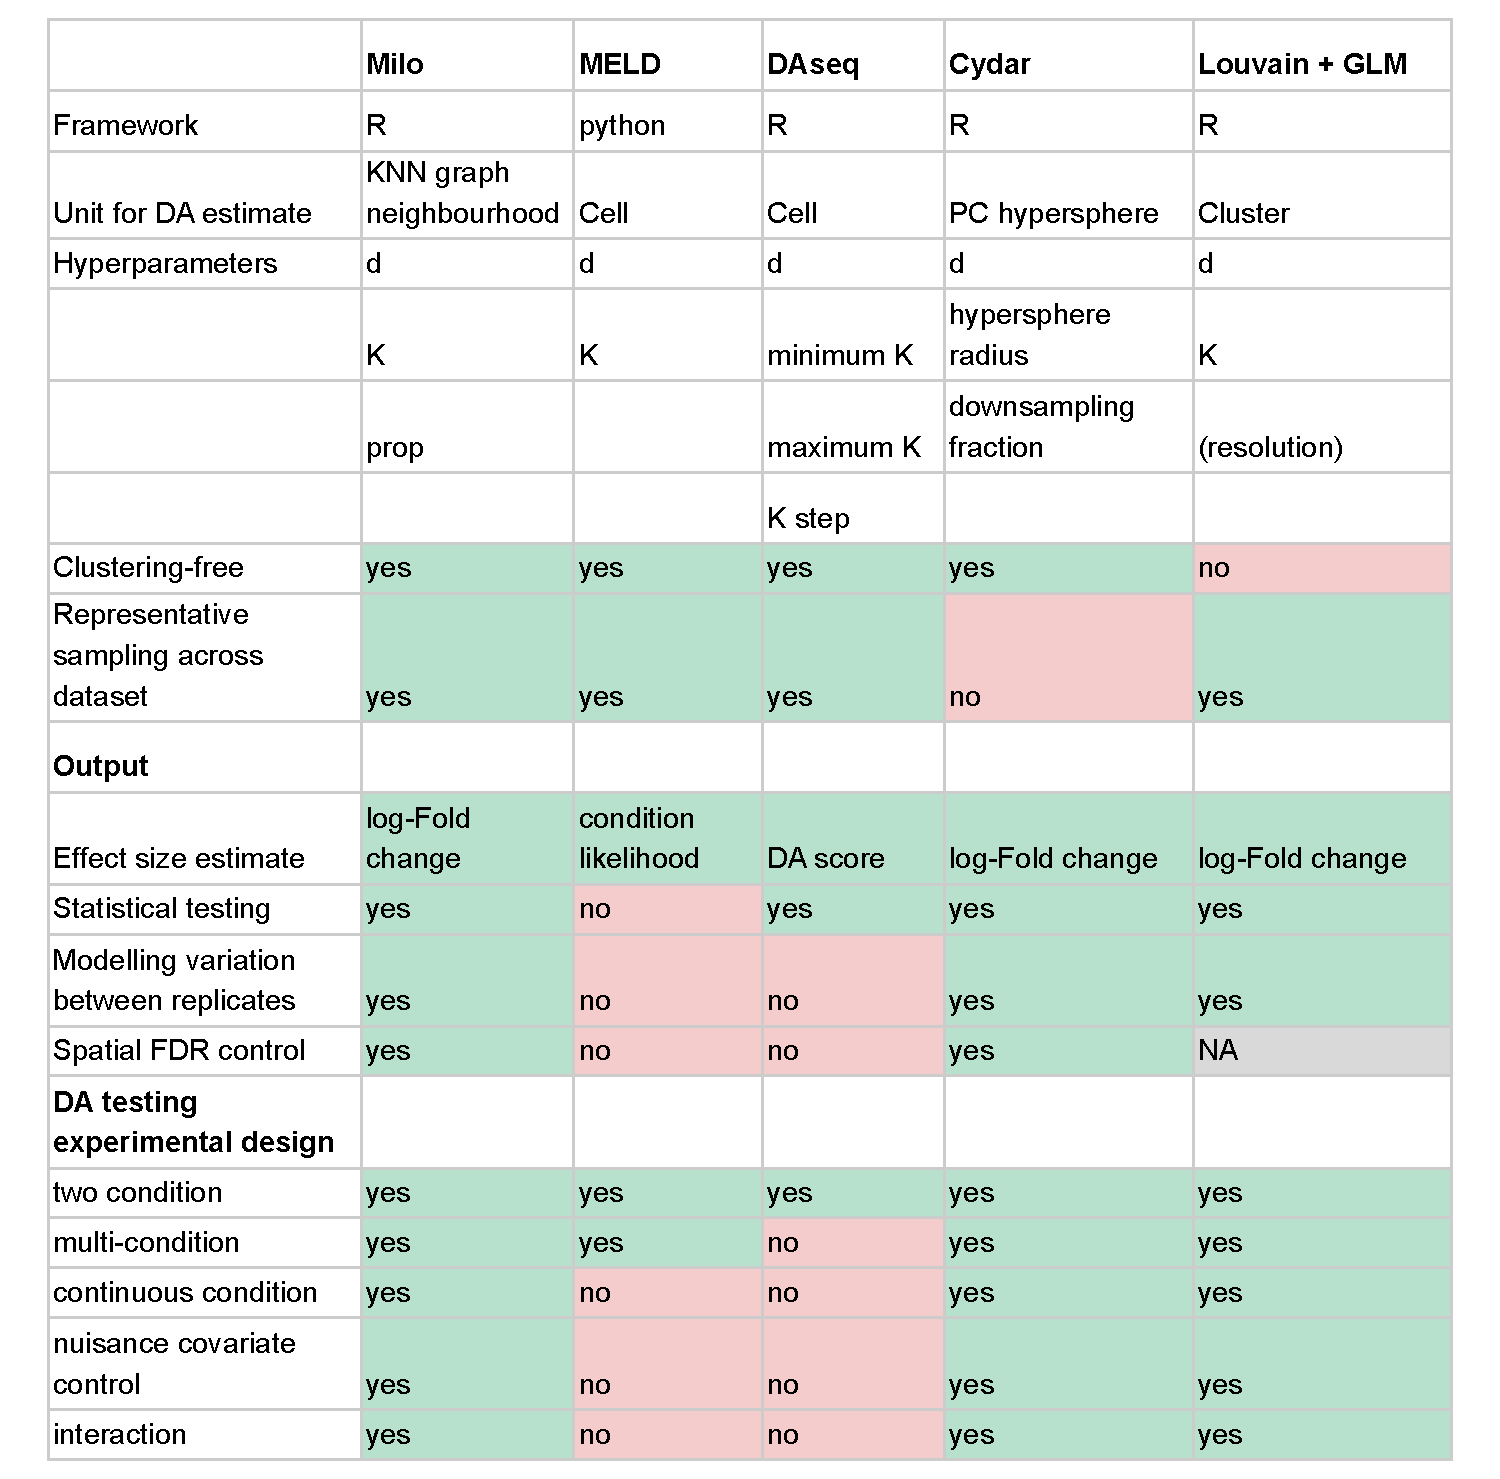
\includegraphics{suppl_tables/table_methods_comparison.pdf}
\caption{\label{fig:sup-tab-1}\textbf{Qualitative comparison of evaluated methods for DA analysis}}
\end{figure}



\begin{figure}
\centering
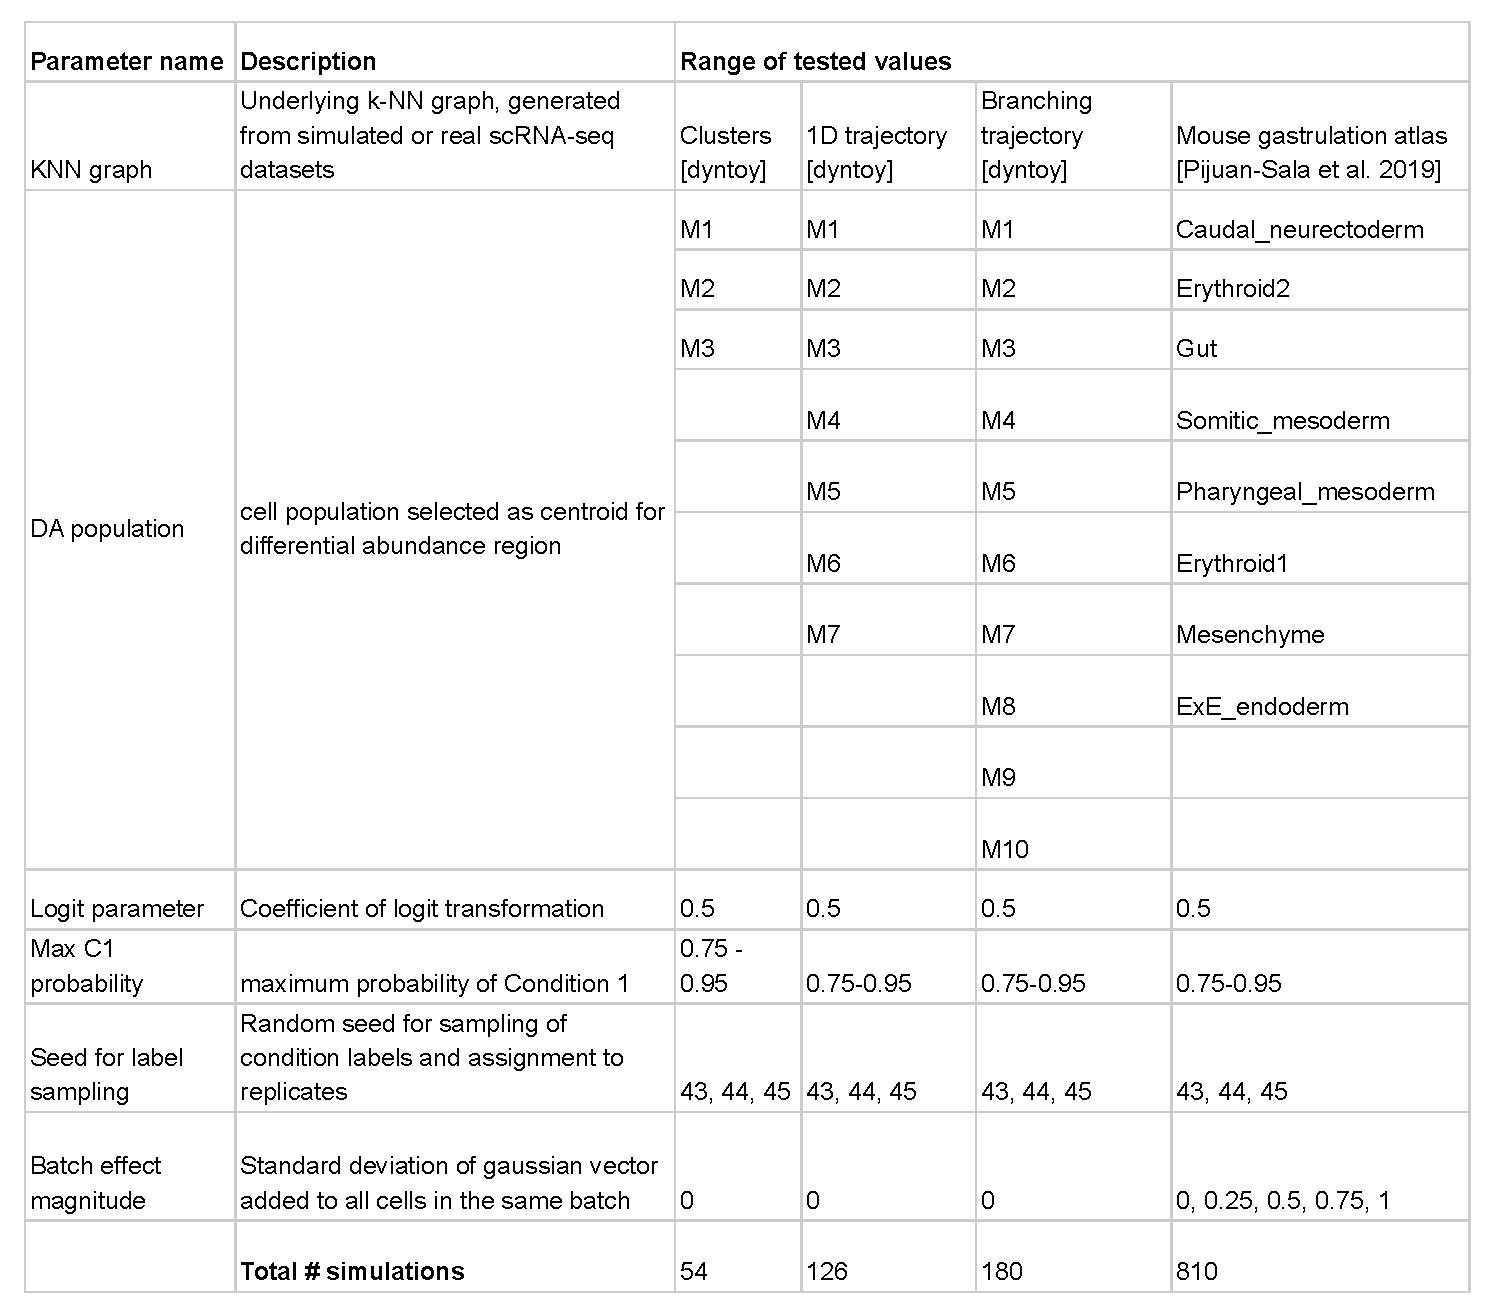
\includegraphics{suppl_tables/table_simulation_params.pdf}
\caption{\label{fig:sup-tab-2}\textbf{Summary of parameters used for DA simulations}}
\end{figure}



\begin{figure}
\centering
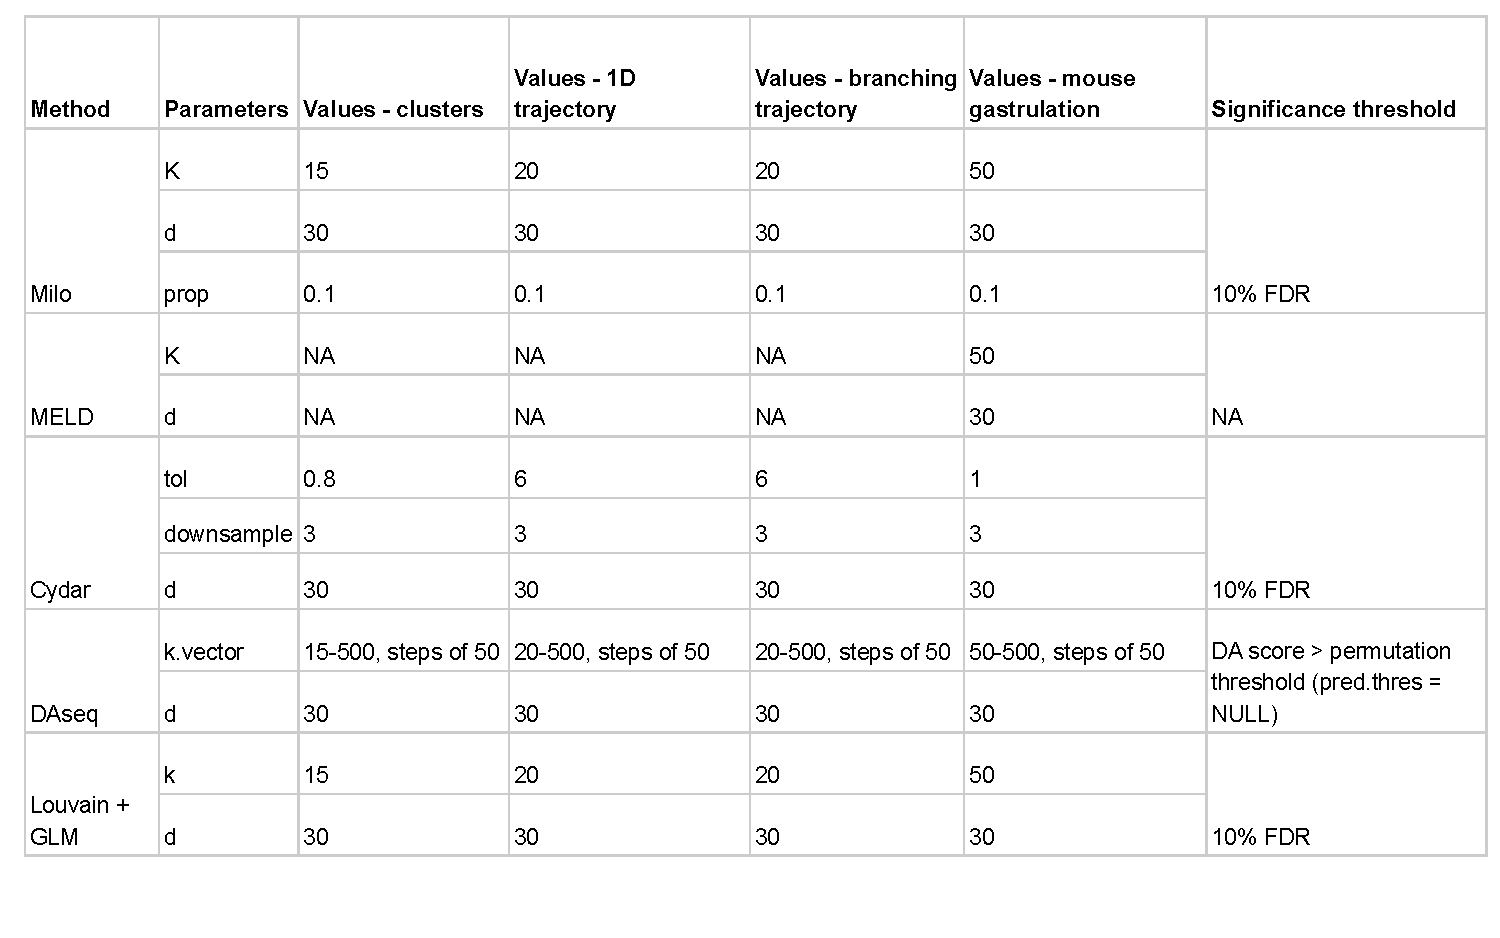
\includegraphics{suppl_tables/table_methods_params.pdf}
\caption{\label{fig:sup-tab-3}\textbf{Summary of parameters used for benchmarking of DA methods}}
\end{figure}



\newpage

\end{document}
